% Template for PLoS
% Version 1.0 January 2009
%
% To compile to pdf, run:
% latex plos.template
% bibtex plos.template
% latex plos.template
% latex plos.template
% dvipdf plos.template

\documentclass[10pt]{article}

\usepackage{graphicx}
\usepackage[space]{grffile}
\usepackage{latexsym}
\usepackage{amsfonts,amsmath,amssymb}
\usepackage{url}
\usepackage[utf8]{inputenc}
\usepackage{fancyref}
\usepackage{hyperref}
\hypersetup{colorlinks=false,pdfborder={0 0 0},}

% cite package, to clean up citations in the main text. Do not remove.
\usepackage{cite}

% Use doublespacing - comment out for single spacing
%\usepackage{setspace} 
%\doublespacing



% Text layout
\topmargin 0.0cm
\oddsidemargin 0.5cm
\evensidemargin 0.5cm
\textwidth 16cm 
\textheight 21cm

% Bold the 'Figure #' in the caption and separate it with a period
% Captions will be left justified
\usepackage[labelfont=bf,labelsep=period,justification=raggedright]{caption}

% Use the PLoS provided bibtex style
\bibliographystyle{plos2009}

% Leave date blank
\date{}

\pagestyle{myheadings}
\begin{document}

% Title must be 150 characters or less
\begin{flushleft}
{\LARGE
\textbf{Adaptive Radiation in Fluctuating Environments}
}
% Insert Author names, affiliations and corresponding author email.
\\
Thomas LaBar$^{1}$, Luiz Irber$^{2}$, Prateek Shetty$^{3}$
\\
{\bf 1} Michigan State University
\\


{\bf 2} Michigan State University
\\
{\bf 3} Michigan State University
\\
\end{flushleft}

% Please keep the abstract between 250 and 300 words




\section{Abstract}

\indent One of the main goals of ecology and evolutionary biology is to understand why there is such an abundance of biological diversity. One of these processes is adaptive radiations, where a species rapidly occupies many ecological niches, triggering a burst of speciation. Most experimental studies of adaptive radiation maintain a constant level of environmental productivity, and find that diversity is maximized at some intermediate productivity level. However, over long timescales, environments are not constant, and productivity fluctuates. Here, we investigated the effect of environmental productivity fluctuations on species diversity using a digital evolution system. We find that for fluctuations less than 10 generations long, diversity is the same as in a high-productivity constant environment. However, for fluctuations of 100 generations or longer, diversity is generated at the same rate as in a low-productivity constant environment. These results hold whether all resource fluctuate synchronously, or separate groups of resources fluctuate together. Our results illustrate the lack of a strong effect of environmental fluctuations on speciation on macroevolutionary timescales

\section{Introduction}
A central problem in ecology and evolutionary biology is understanding how species diversity is generated and maintained. One of the theories to explain how diversity is generated on macroevolutionary timescales is the ecological theory of adaptive radiations \cite{schluter2000ecology}. An adaptive radiation occurs when a single evolutionary lineage diversifies into a multitude of species. Rapid diversification occurs after a species colonizes an area with many unoccupied ecological niches. Resource competition causes phenotypic differentiation, and then speciation, to occur \cite{schluter2000ecology}. Most of science's illustrative examples of past adaptive radiations come from eukaryotic species visible to the human eye; these include the Galapagos finches \cite{grant2011and},
the Anolis lizards \cite{losos2009lizards}, and the Great African lake cichlids \cite{seehausen2006african}. However, the complexity of natural ecosystems and the limited number of examples demonstrate a need for simple model systems to understand the range of processes that drive adaptive radiations.

In order to overcome the limitations facing the study of evolutionary phenomena in nature, scientists utilize both microbial and digital evolution experiments \cite{kawecki2012experimental}.
By studying systems that still contain the essence of biological systems in nature, but with less complexity, it may be easier to formulate and test hypotheses, and establish a general theory of adaptive radiations \cite{kassen2009toward}.
In the field of microbial evolution, Pseudomonas fluorescens has been established as the model organism for the study of adaptive radiations, due to its ability to rapidly diversify \cite{spiers2002adaptive}.
Additionally, some other studies have used the model organism Escherichia coli due to its use in long-term evolutionary studies \cite{rosenzweig1994microbial,friesen2004experimental,le2012ecological}.
Due to the fast generation times of microbial systems, it is possible to investigate questions such as the effect of spatial heterogeneity on diversification \cite{rainey1998adaptive}, the role of productivity and disturbance on diversification (\cite{kassen2000diversity}, \cite{buckling2000disturbance,kassen2004ecological}, and the role of predation on adaptive radiations \cite{meyer2007effects}.
Meanwhile, in digital systems, studies have shown adaptive radiation occurs in a well-mixed environment due to negative frequency-dependent selection \cite{chow2004adaptive}.

Most, although not all, work in evolution experiments maintain a constant abiotic environment throughout the experiment (Collins 2010).
However, organisms do not live in constant environments.
Since the ecological theory of adaptive radiations claims diversification occurs due to resource competition \cite{schluter2000ecological}, it follows that fluctuations in resource availability may effect diversity generation.
Additionally, previous work in both microbial and digital systems showed that diversity is dependent on resource availability in constant abiotic environments (\cite{kassen2000diversity}, \cite{chow2004adaptive}.
Previous work on microbial experiments concerning diversification in non-constant environments (reviewed in \cite{kassen2002experimental,kassen2009toward} ) includes explorations of the effect of temporal grain on diversity \cite{venail2011diversification}, the effect of fluctuating environments on landscape structure \cite{cooper2010experimental}, and the evolution of cost-free generalism in fluctuating environments \cite{buckling2007experimental}.
Although research in digital systems explored the effects of fluctuating environments on evolutionary outcomes, very few impose a resource-based ecology needed to study adaptive radiations \cite{li2004digital,clune2007investigating,misevic2010experiments}.
However, to our knowledge, no paper has investigated adaptive radiation under resource availability fluctuations.

Here, we extend previous work that investigated adaptive radiation in a constant environment with the digital evolution platform Avida \cite{chow2004adaptive} by fluctuating environment productivity.
We varied resource inflows between a rate that allowed for high diversification, and a rate that resulted in low diversification.
We show that fluctuating resource inflows do not increase diversity.
Moreover, species richness itself does not fluctuate, no matter the fluctuation duration.
At fluctuations that occur from within a generation to a couple of generations, the populations diversifies at the same rate as it would in a constant, high inflow, environment.
At fluctuations lasting many generations, populations diversify as they do in constant, low inflow, environments.
Furthermore, the gain and loss of high levels of resource consumption prevented diversification.
These results were constant for scenarios when all resource inflows fluctuate in synchrony, or groups of inflows fluctuated at different times. 

\section{Methods}

\subsection{Avida Overview}
To test the effects of fluctuating environments on adaptive radiations, we used the digital evolution platform Avida v2.13.0 \cite{ofria2009avida}.
This tool has allowed researchers to investigate hypotheses that are difficult or currently impossible to test in biological systems, such as the origins of biological complexity \cite{adami2000evolution,lenski1999genome}, the evolution of complex features \cite{lenski2003evolutionary}, and the role of deleterious mutations in adaptation \cite{covert2013experiments}.
In Avida, computer programs, referred to as Avidians, compete for CPU time and memory. These programs consist of a circular genome of instructions, including some instructions, known as the copy loop, that allows for self-replication.
These instructions form a Turing-complete language, allowing for individuals of great complexity.
Avidian reproduction consists of an individual copying its genome and placing the copy of itself into a new memory location.
There are limited memory locations in Avida, so individuals face a strong selective pressure to reproduce as quickly as possible in order to occupy the limited memory.
However, when Avidians reproduce, the copying process is error-prone; this introduces mutations in an offspring's genome.
Offspring may contain genomes different than their parents due to various experiment-dependent types of mutations.

Over time, Avidians, through mutation and selection, can also evolve the ability to perform certain boolean logic tasks, such as NAND and EQUALS.
The ability to perform these logic tasks, of which there are usually nine, can be thought of as a primitive digital metabolism.
When organisms perform such tasks, they are rewarded by increasing their speed of replication.
This results in a selective advantage for organisms that can perform these tasks, and leads to them quickly spreading throughout the population.
These tasks also build on each other; an individual that performs NAND may later co-opt that task to perform equals.
In some experiments, limited resources are also associated with each logic task, introducing frequency-dependent selection into the environment.
Since Avidians have error-prone replication, heritability, and their success in the environment is based on their genome, these computer programs undergo the same Darwinian evolutionary process that biological organisms experience. 

\subsection{Experimental Setup}

We used the limited-resource environment, and a similar experimental setup, from \cite{chow2004adaptive}.
This is a nine resource environment, where each of the nine default logic tasks corresponded to its own resource.
Each time a task was performed, the organisms would consume the minimum of either 5 units of resource, or 0.0025 percent of the total resource availability.
Organisms could perform each task an unlimited number of times.
The population was seeded with the default 100 instructions-long genome that could self-replicate, but could not perform any logic tasks.
The population was well-mixed, i.e., offspring would be placed randomly in the population, and resources were globally available, to mimic chemostat conditions.
The population was capped at 3000 individuals, and the experiments ran for 400,000 updates (the unit of time in Avida, where one update is such that each individual, on average, executes 30 instructions).
We ran 30 replicates for each experimental treatment.

In order to create a fluctuating environment, we designed the experiments so resource inflow would change throughout the experiments. In previous research, resource inflow was constant and ranged among seven orders of magnitude between the different experimental treatments. Here, we varied resource inflow between 100 units per update per resource, and 1 unit per update per resource. Because there are many ways for resource inflows to fluctuate, We used two different treatments of environment fluctuations: synchronous and staggered. During synchronous resource fluctuations, all nine resource inflows would either increase to an inflow rate of 100 units, or decrease to an inflow rate of 1 unit. During staggered resource fluctuations, one set of resources (those associated with the not, and, andn, and nor tasks) would inflow at one rate, and another set of resources (those associated with the nand, orn, or, and xor tasks) would inflow at the other rate. In this fluctuation regime, the resource associate with equ would always inflow at the high rate of 100 units. To look at the effect of different fluctuations lengths, we ran experiments for both synchronous and staggered fluctuations with fluctuation lengths ranging from $10^0$ updates to $10^5$ updates. Since we often collected data only at the end of a run, we ran a set of synchronous fluctuation experiments starting with all resources inflowing at the high rate at the beginning, and another set with all resources inflowing at the low rate. This would allow us to analyze the data for experiments ending at the low inflow rate, and ending at the high inflow rate, respectively.

\subsection{Clustering Algorithm}

One way of finding species in a population is by clustering organisms
based on a distance function.
The function chosen by \cite{chow2004adaptive} in their
clustering algorithm was the phylogenetic distance, which counts the
number of steps in the line of descent from the most recent common ancestor
between two organisms. Other functions were discarded because they
lumped organisms with important phenotypic differences into the same species
(Hamming distance) or split organisms with identical phenotypes into
different species (time-to-most-recent-common-ancestor).

In order to form clusters the algorithm successively calculates the minimum
phylogenetic distance between organisms and sum it. When the difference
between sums of previous and current iteration is greater than a cutoff
value $c$ the organism is chosen as the center of a cluster. Other organisms
are chosen based on the distance to the central organism.
We used the same cutoff value $c$ from \cite{chow2004adaptive}.

\subsection{Data Analysis}

We used Avida's analyze mode to calculate organism statistics. We performed other data analysis with Python modules SciPy \cite{oliphant2007python}, and created plots with matplotlib \cite{hunter2007matplotlib}.
An organism's phylogenetic depth, displayed in the flame graph, was calculated as the number of ancestors that possessed a different genome from its parent.
All error bars are 95\% confidence intervals unless otherwise stated.

\section{Results}

\subsection{Species Richness}

We found that species richness was not greater in any fluctuating environment than in a constant environment (Fig.1). Additionally, all fluctuations types resulted in similar levels of species richness. For short fluctuation lengths (<1000 updates), species richness ranges from 3 to 3.5 species. For longer fluctuations, species richness ranged from 1 to 2 species. Species richness eventually saturated over time in both synchronous (Fig.2) and staggered (Fig.3) fluctuation environments.

\subsection{Resources Levels}

For short synchronous fluctuations and for all staggered fluctuations, total resource levels were drawn down to a very low level, indicating either the resource was inflowing at a low level, or it was being consumed at a high level (Fig.4). The lack of fluctuations indicate that organisms were not abandoning the ability to consume resources at high amounts. This result does not hold for long, synchronous fluctuations. This indicates that individuals were abandoning and regaining the ability to consume resources, as there was a lag time between the beginning of high resource inflow, and the consumption of those resources.

\subsection{Task Performance}
To see whether populations failed to diversify due to changes in task performance, we examined the total number of tasks performed in the last fifty thousand updates (Fig. 5).In an environment with synchronous fluctuations, Avidians performed between 2000 and 10,000 tasks, dependent on resource inflow and fluctuation length. In the staggered environment, the populations performed between 7,000 and 13,000 tasks, with most treatment populations performing greater than 11,000 tasks. Avidians in the synchronous, long fluctuation environments would lose the ability to perform tasks in low resource conditions and would subsequently re-evolve them in high resource conditions. The same phenomenon was observed in staggered conditions too, but it was much less pronounced.

\section{Discussion}

Here, we tested the effects of different fluctuating productivity environments on final species richness in a digital evolution system. We found that fluctuating resource inflow did not increase species richness. At short fluctuating lengths, the community attained a level of species richness similar to that found when resources inflowed at a high rate of productivity \cite{chow2004adaptive}. Meanwhile, at long fluctuation lengths, the resultant species richness was equivalent to the scenario where resources inflowed at a low productivity level \cite{chow2004adaptive}. The transition from a diverse community to a community with one species occurred somewhere between fluctuations of length 100 updates and 1000 updates; this was equivalent to 10-100 generations, dependent on the type of fluctuation. Finally, we show that the population loses and reacquires the ability to consume resources at long fluctuations; this suggests a reason for why diversification does not occur at these fluctuation levels.

Previous results examining the role of temporal environmental variation on diversity are mixed, and studies show that temporal variation can result in increased or decreased diversity (reviewed in \cite{kassen2002experimental}). In microbial experiments, there is evidence that genotypic diversity is maximized at intermediate fluctuation lengths \cite{venail2011diversification}. There are also examples where only a single niche specialist evolves \cite{jasmin2007evolution}, and where only a single generalist evolves \cite{reboud1997experimental} in temporally-fluctuating environments. We have shown that diversity does depend on the length of the environmental variation (sometimes referred to as the grain). However, we did not find that intermediate fluctuations resulted in maximum diversity; instead, short fluctuations caused the highest level of species richness (Fig. 1). At these short fluctuation lengths, individuals may not have enough time to lose the ability to consume resources at the high inflow level (Fig. 4), and thus would retain the ability to do so once the environments changes back to a high productivity level. This would maintain negative frequency-dependent selection long enough for diversity to be maintained in the population.

Many previous studies either design the abiotic environment to fluctuate between two resources (i.e. \cite{cooper2010experimental}). Other studies, when they vary productivity, look at the evolution of the population's fitness, but do not focus on phenotypic diversification (i.e. \cite{buckling2007experimental}). These studies often find a lack of a cost to being a generalist \cite{kassen2002experimental}. Our study focused on adaptive radiation in a varying productivty environment with many resources, where generalists still evolve even in a constant environment \cite{chow2004adaptive}. However, generalists almost always evolve in the low productivity environment, but less often in the high productivity environment (see Fig.6 in \cite{chow2004adaptive}). This also explains the high diversity when fluctuations are short; generalists are not under pressure to evolve, unlike when fluctuations are longer, and individuals spend more consecutive time in a low-productivity environment. In these low-resource environments, there are not enough resources to specialize on any resource.

Our work only explored two types of non-constant abiotic environments: one where all resources fluctuated together between a high inflow level and a low inflow level, and another where two groups of resources fluctuated, with one group at the high inflow level, and the other at the low inflow level. Natural environments may not fluctuate in such a constant manner. The final species richness may change if resources fluctuate between being present or absent, as in other work \cite{cooper2010experimental}, or if resource inflow pulses, as it does in some ecosystems \cite{holt2008theoretical}. Finally, fluctuation lengths were set up for a number of updates; it may be better to control fluctuations by a number of generations, as generations passed in this experiment was not constant across fluctuation lengths and fluctuation types. 

Here, we explored the effect of a non-constant environment, one where environmental productivity fluctuates, on the final species richness in an adaptive radiation. We found that the final species richness was dependent on the length of the resource fluctuation; short fluctuations led to high species richness, and long long fluctuations usually led to communities with only one species. However, there are many types of non-constant environments, and we feel this digital evolution system is ideal for future exploration. For example, it would be interesting to explore an environment where resources did not fluctuate constantly; for example, an experiment could be set up where resource pulse into the environment with some frequency, or where only one random resource inflows into the environment at a time. Exploring the effects of spatial heterogeneity should also prove interesting, as spatial heterogeneity is expected to enhance diversity to a greater extent than temporal heterogeneity \cite{kassen2002experimental}. Such further studies would solidify our understanding of processes that affect adaptive radiations and shape diversity across ecological communities.

\bibliography{bibliography/converted_to_latex.bib}

\begin{figure}[h!]
\begin{center}
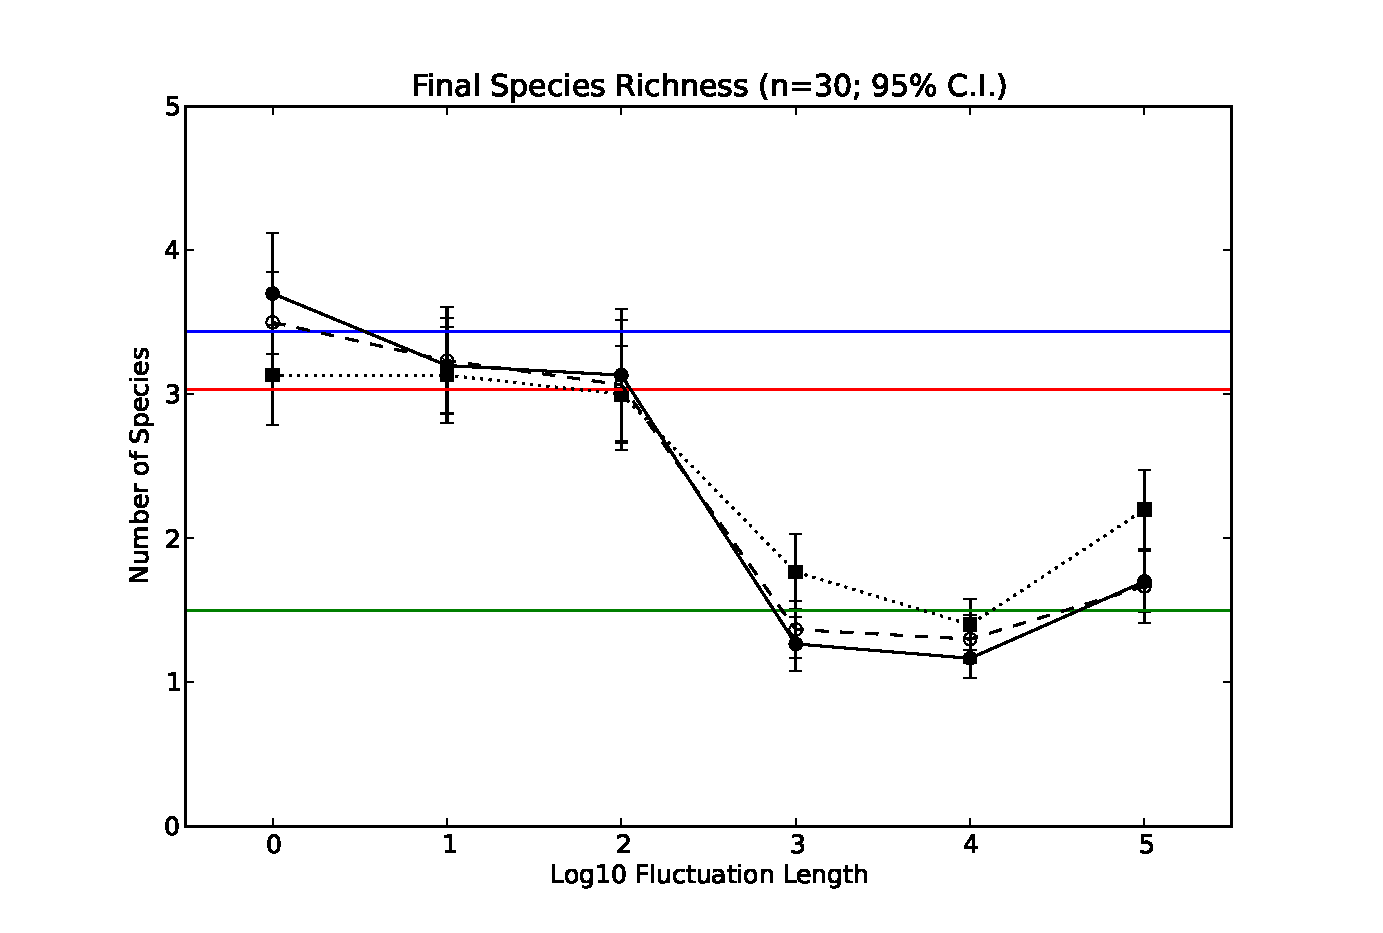
\includegraphics[width=0.7\columnwidth]{figures/fig_1_species_richness2/fig_1_species_richness2.eps}
\caption{Fig.1 Final Species Richness as a function of the number of updates a environmental fluctuation lasts. Solid (open) circles represent synchronous fluctuations that started inflowing at a high (low) level. Solid squares represent staggered fluctuations. Green, blue, red lines represent final species richness for a constant inflow of $1,10,100$ units per update, respectively.}
\end{center}
\end{figure}

\begin{figure}[h!]
\begin{center}
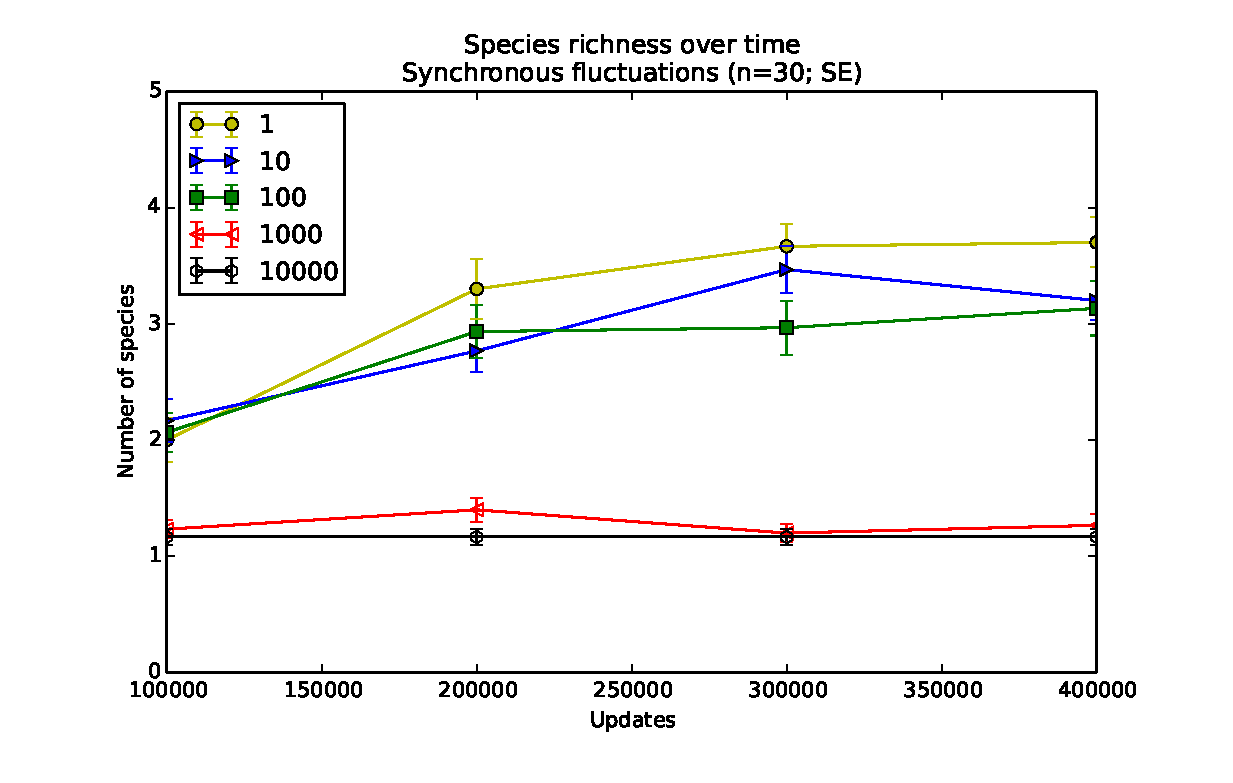
\includegraphics[width=0.7\columnwidth]{figures/synchronous/synchronous.eps}
\caption{Fig. 2 Species richness through time for synchronous fluctuations. Yellow, blue, green, red, black lines represent fluctuations of length $1,10,100,1000,10000$ updates, respectively. Error bars are standard error of the mean.}
\end{center}
\end{figure}

\begin{figure}[h!]
\begin{center}
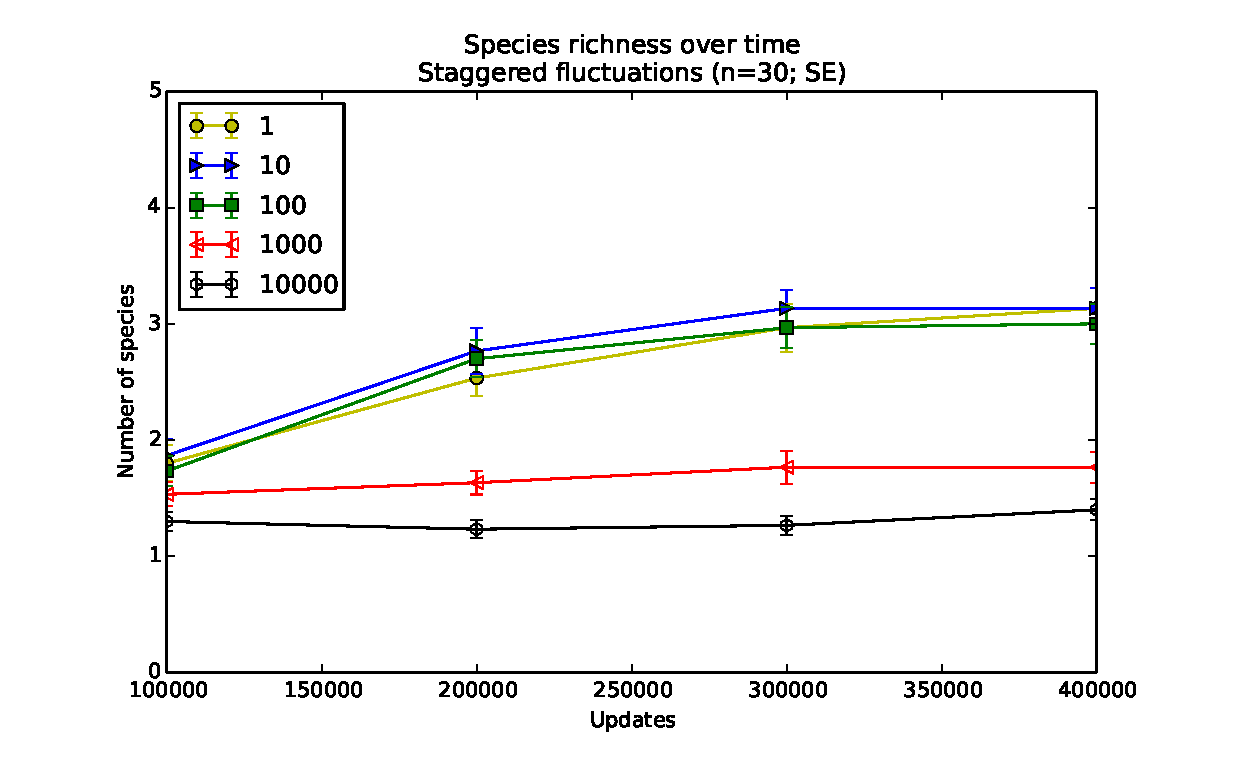
\includegraphics[width=0.7\columnwidth]{figures/staggered/staggered.eps}
\caption{Fig. 3 Species richness through time for staggered fluctuations. Yellow, blue, green, red, black lines represent fluctuations of length $1,10,100,1000,10000$ updates, respectively. Error bars are standard error of the mean.}
\end{center}
\end{figure}

\begin{figure}[h!]
\begin{center}
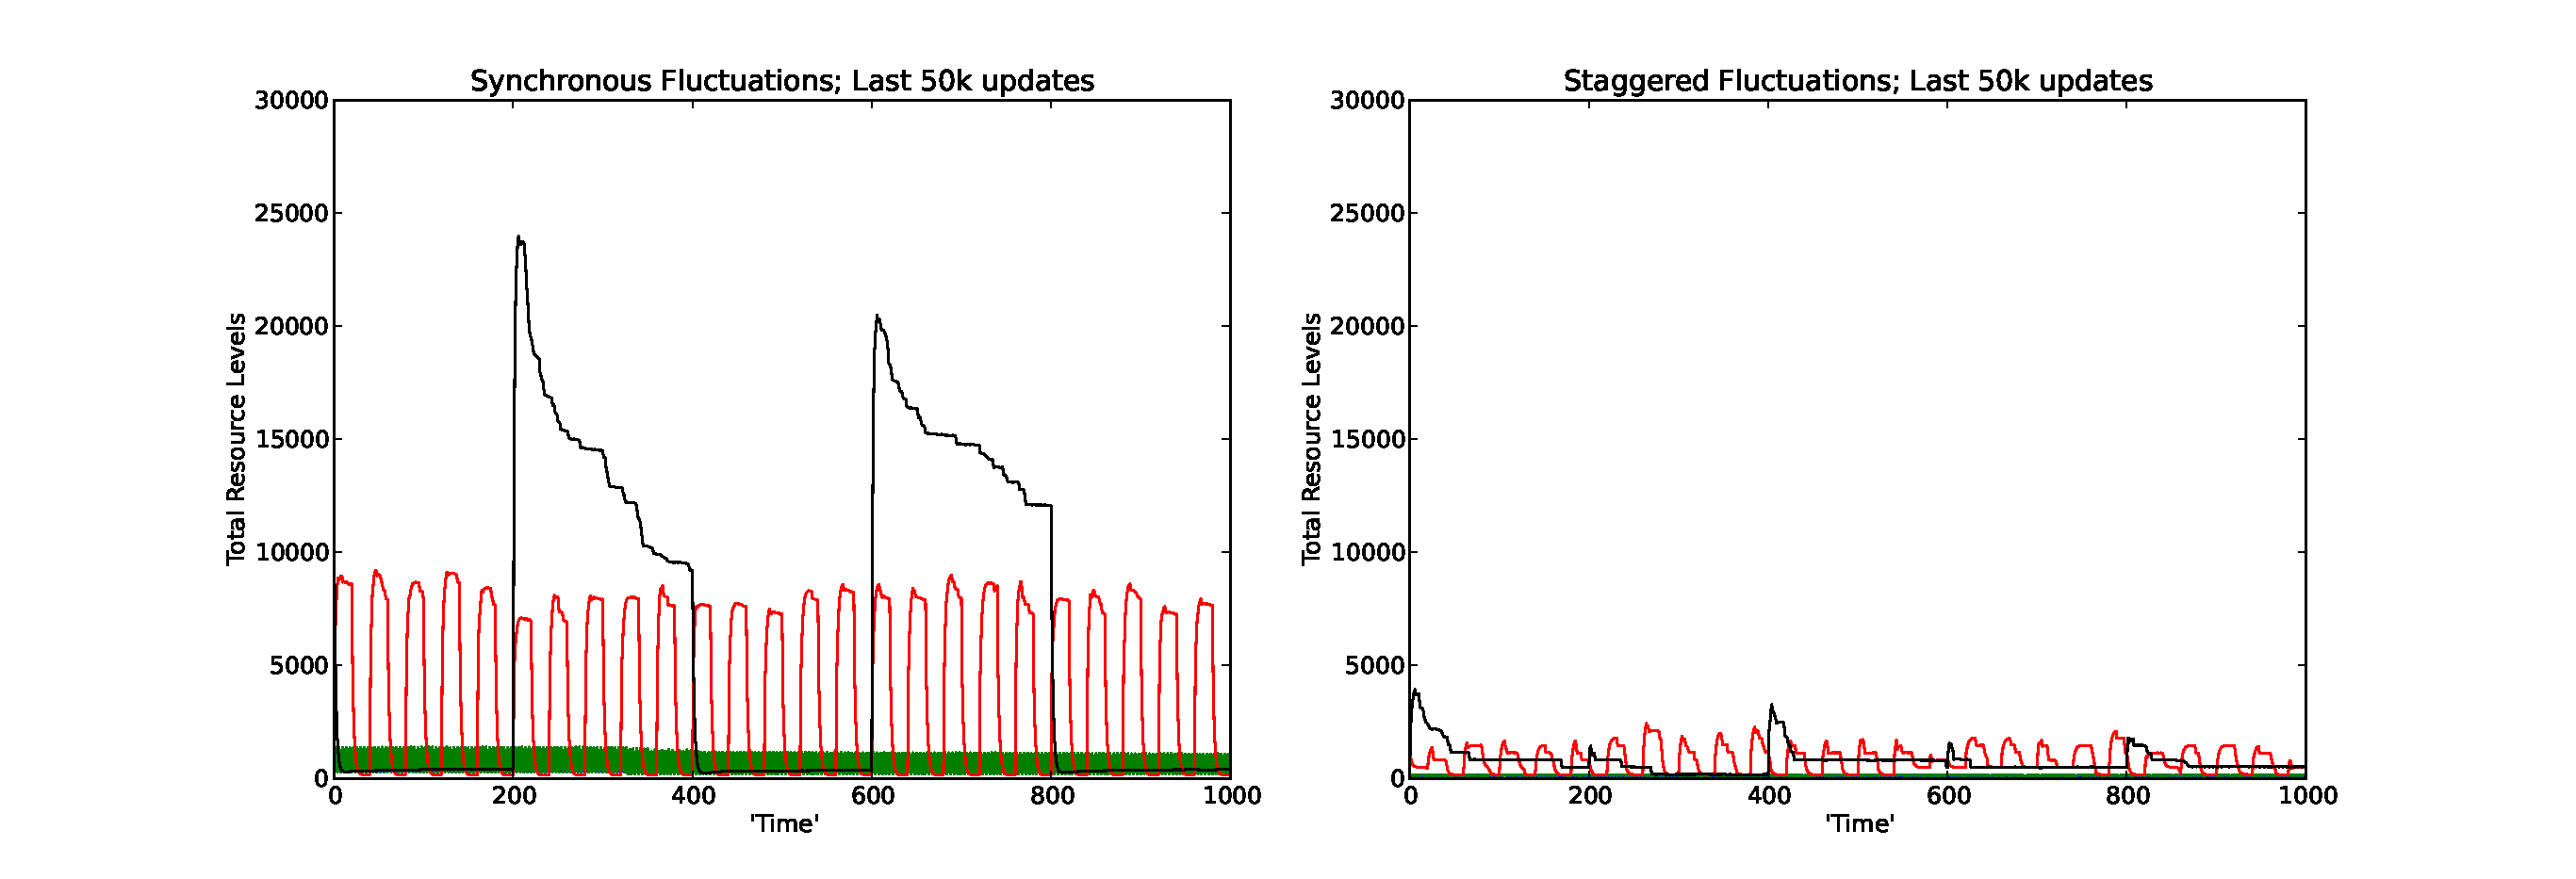
\includegraphics[width=0.7\columnwidth]{figures/fig_3_total_resource_levels2/fig_3_total_resource_levels2.eps}
\caption{Fig. 4 Mean total resource levels across a population across the last $5 \times 10^4$ updates. Left (right) panel shows synchronous (staggered) fluctuations. Yellow, blue, green, red, black lines represent fluctuations of length $1,10,100,1000,10000$ updates, respectively.}
\end{center}
\end{figure}

\begin{figure}[h!]
\begin{center}
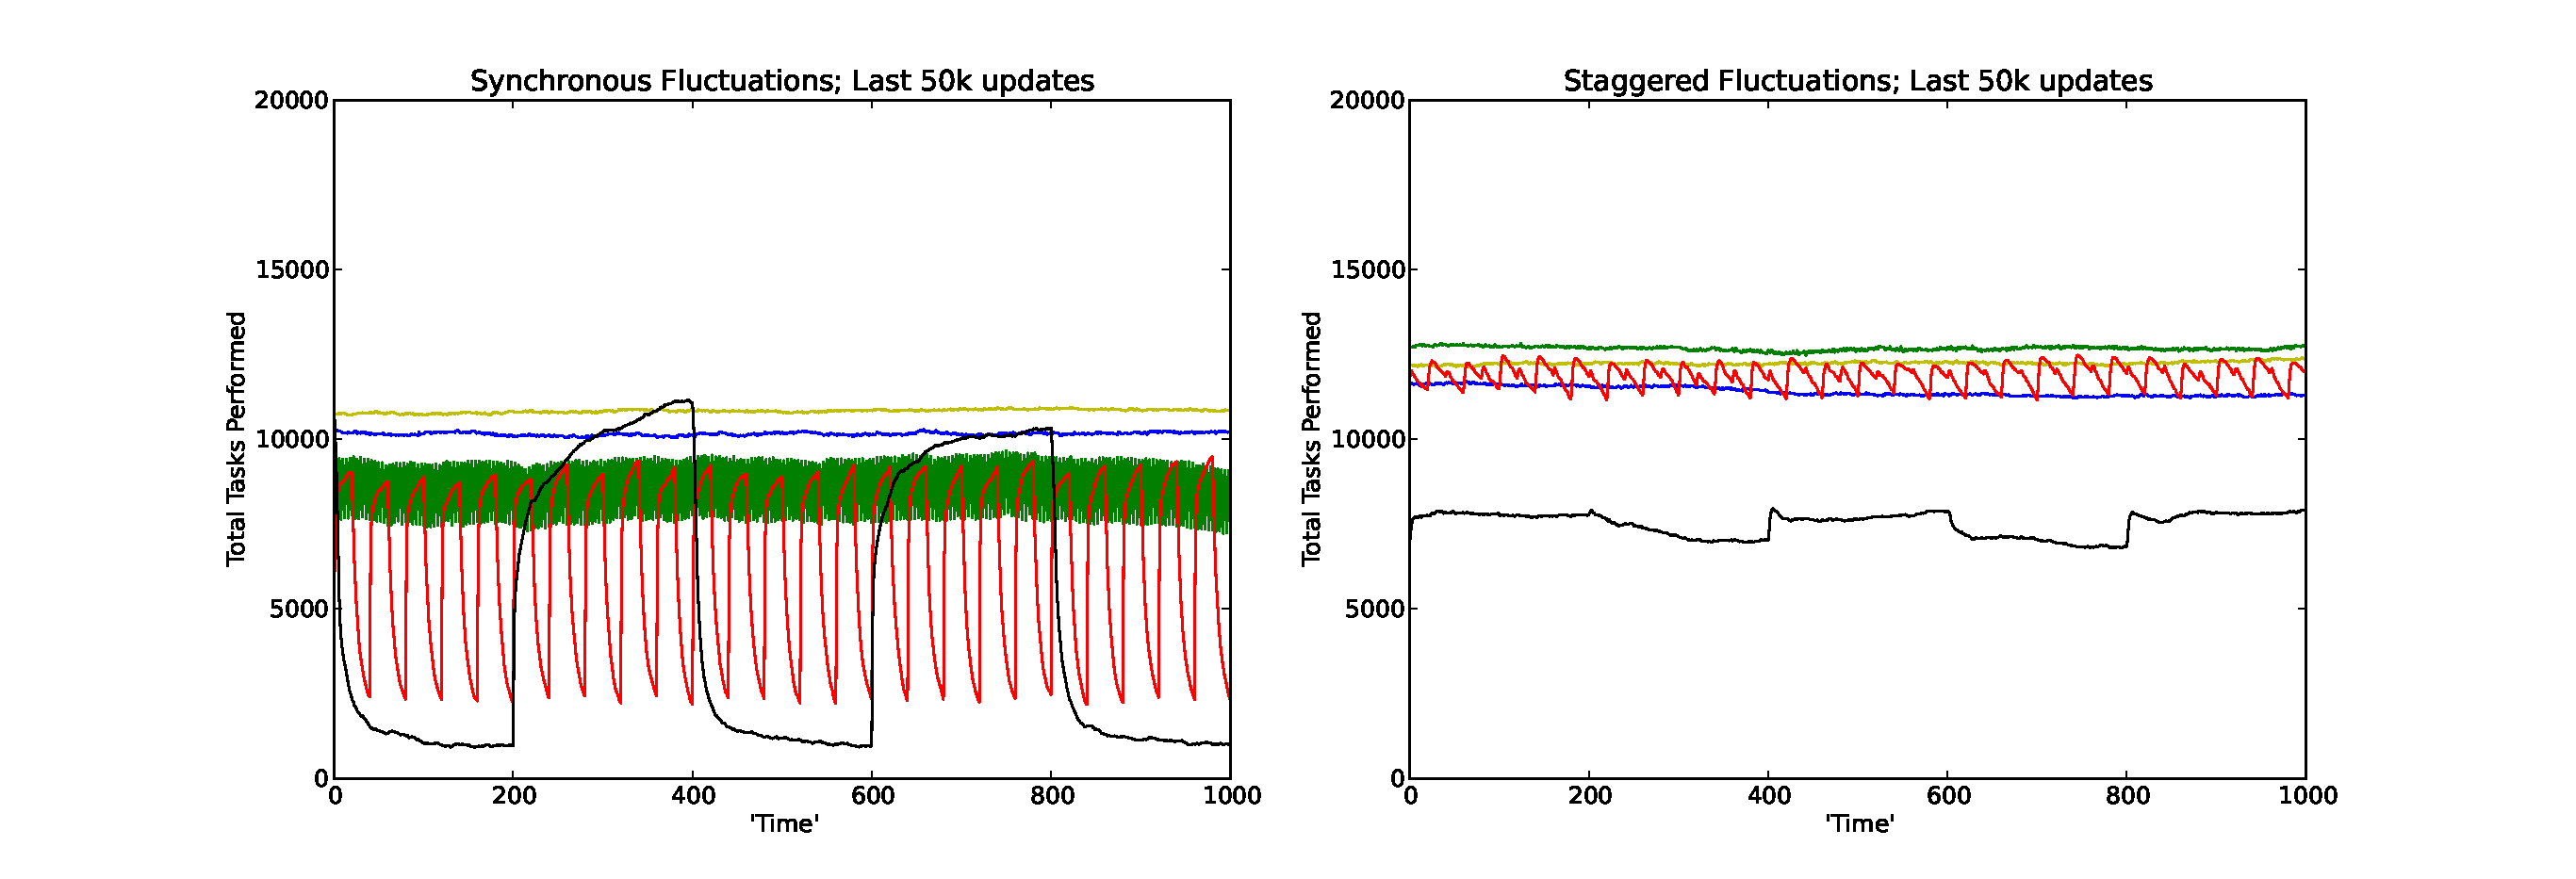
\includegraphics[width=0.7\columnwidth]{figures/fig_2_total_task_performance2/fig_2_total_task_performance2.eps}
\caption{Fig. 5 Mean total number of tasks performed across a population across the last $5 \times 10^4$ updates. Left (right) panel shows synchronous (staggered) fluctuations. Yellow, blue, green, red, black lines represent fluctuations of length $1,10,100,1000,10000$ updates, respectively.}
\end{center}
\end{figure}

\begin{figure}[h!]
\begin{center}
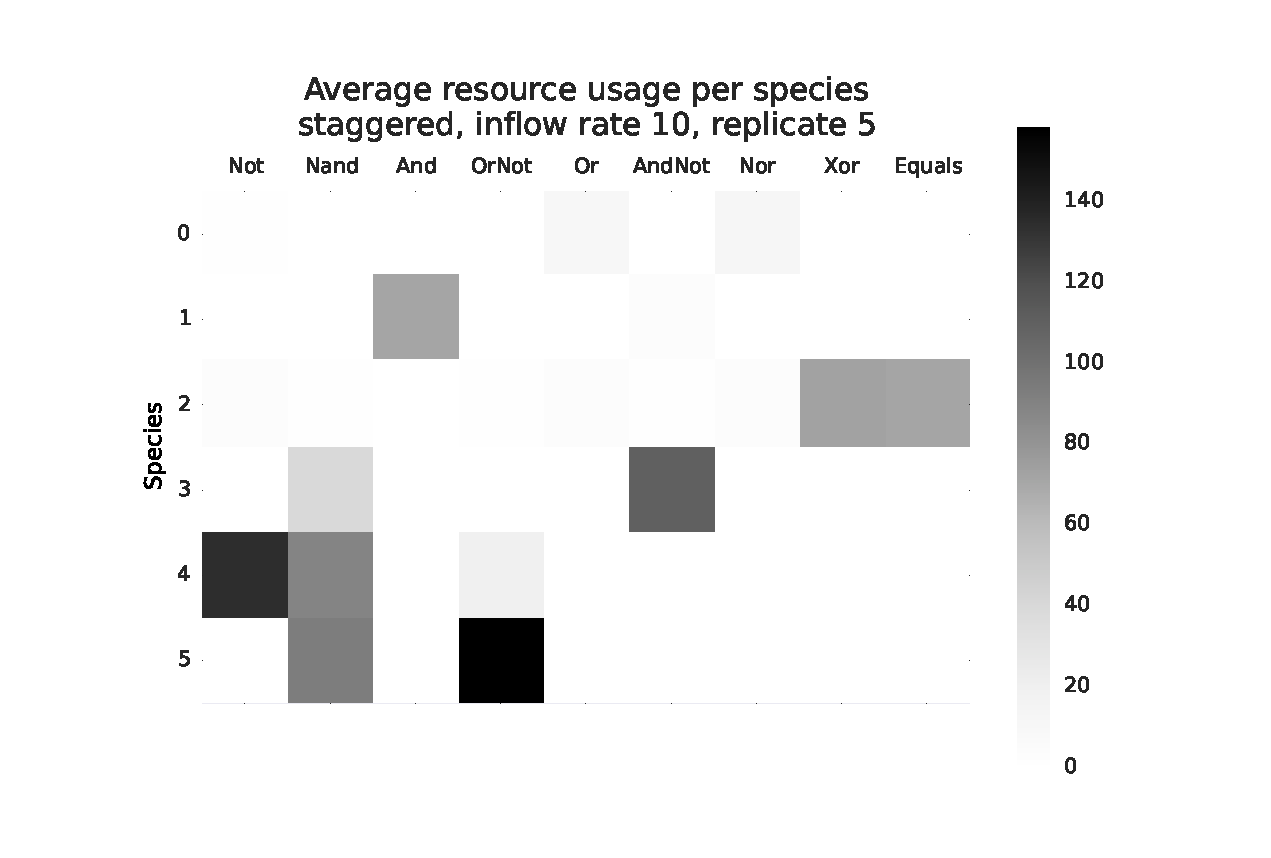
\includegraphics[width=0.7\columnwidth]{figures/heatmap/heatmap.eps}
\caption{Fig. 6 Heat map showing how many times each species performs each task for one replicate. Counts are averaged over the entire species's population.}
\end{center}
\end{figure}


\end{document}

